\begin{comment}
* Labeling details
- UI, filtering strategy
- Statistics
- Payment
- Timing
- Effectiveness

* General model training
- roberta finetuning
- 4 random seeds
- 3 random samples

* Task 1 - sentiment analysis, generalization accuracy
- 
- 
- 

* Task 2 - NLI, challenge set

* Task 3 - QQP checklist

\end{comment}

\section{Application 1: Data Collection}
\ref{sec:app_label}

\subsection{Annotation Procedure}

\begin{figure}[t]
\centering
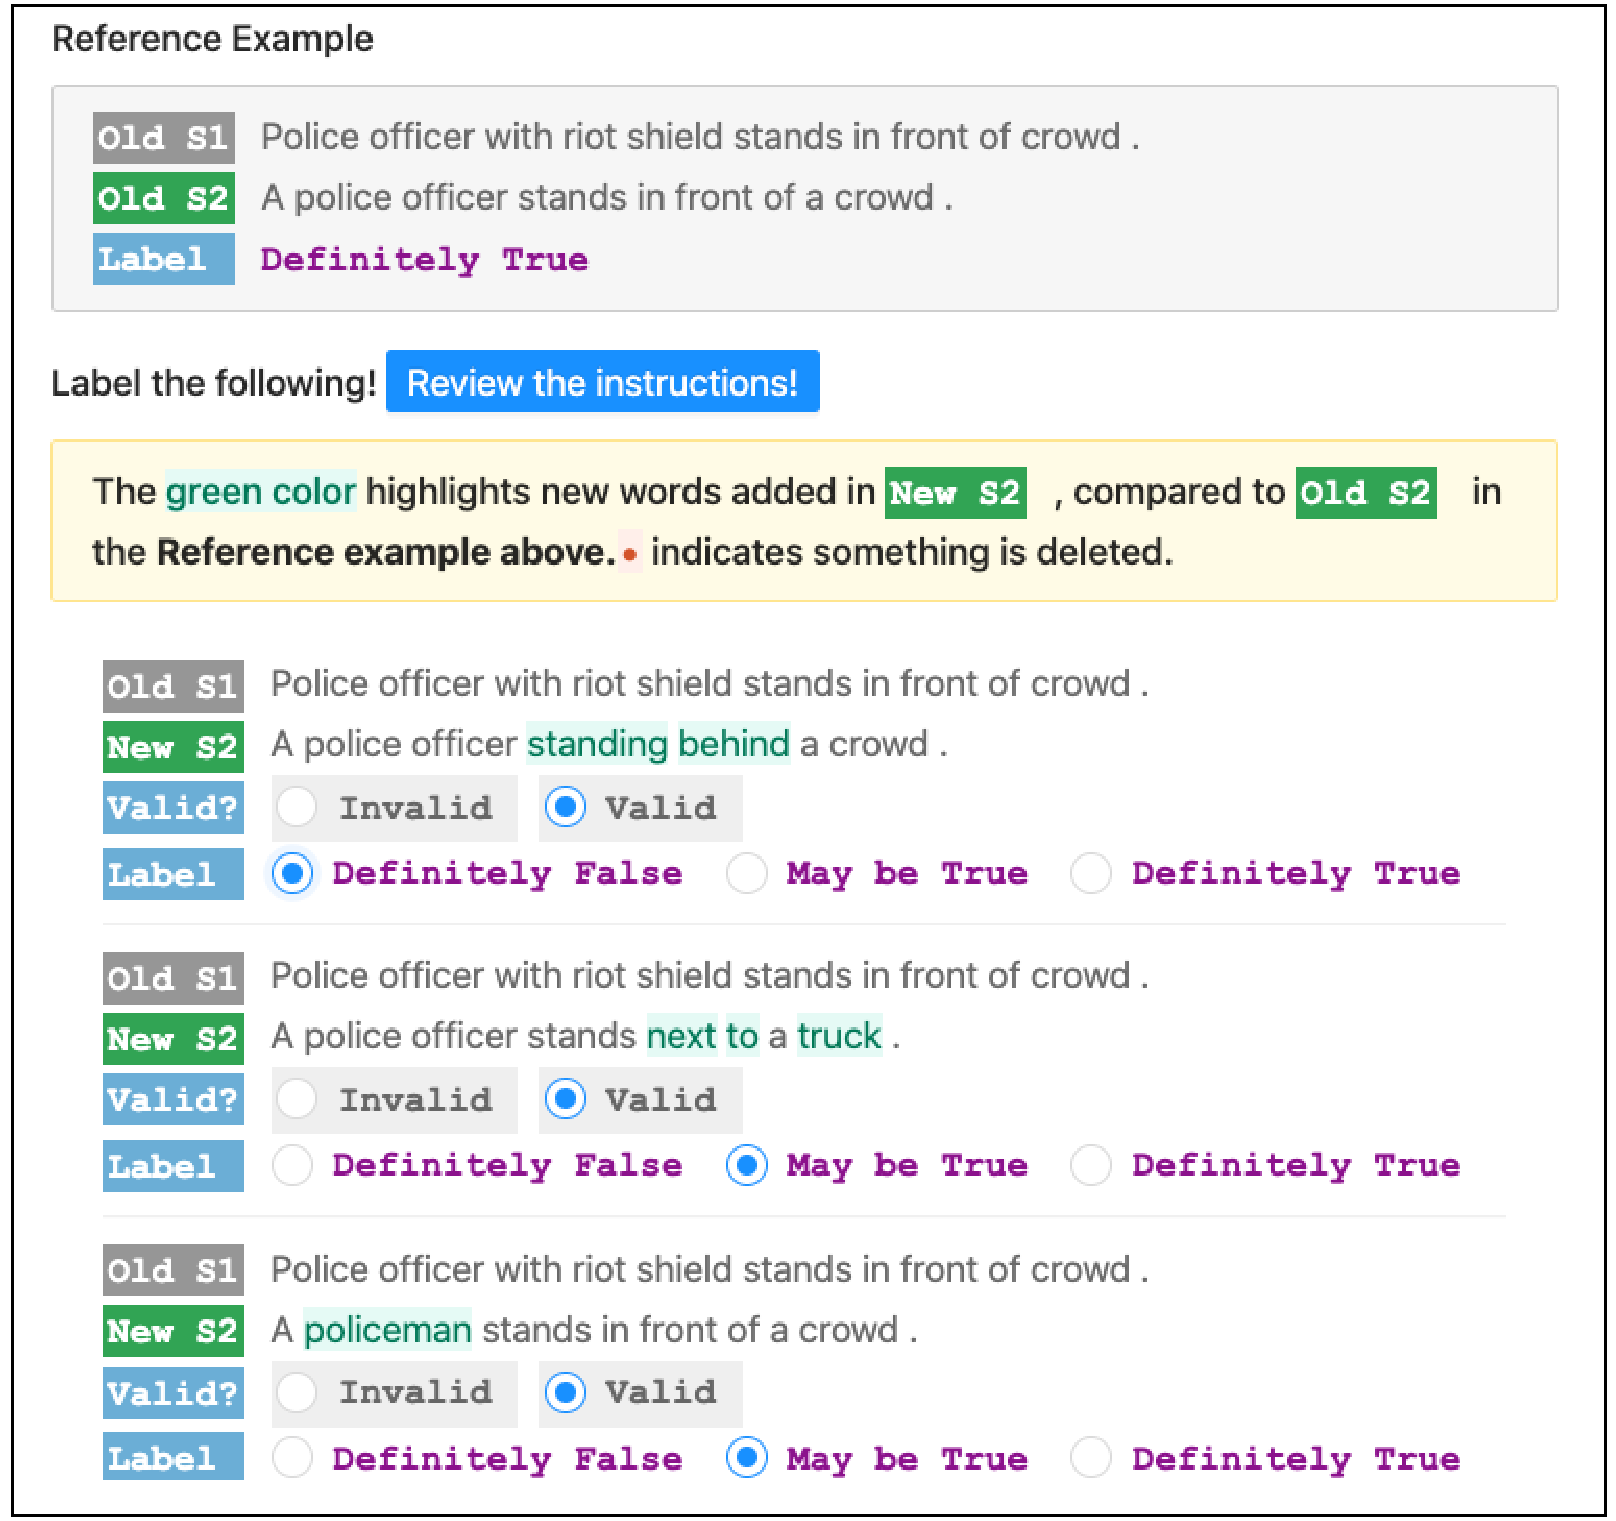
\includegraphics[width=1\columnwidth]{figures/mturk_label}
\vspace{-15pt}
\caption{A sample labeling task. For each round of labeling, the annotator is given the original instance (and its label) as a reference, and they are tasked to label three variations of the instance by (1) grammatically validity and (2) classification task label. A more detailed instruction is in \S\ref{appendix:label_instruct}. \wts{This is placeholder screenshot. Change width/height ratio, choose a better example}}
\vspace{-10pt}
\label{fig:mturk_instruction}
\end{figure}

\subsection{Counterfactual Data Augmentation}

\begin{comment}
For testing on other datasets, we use a random subset (2000 examples) of the test sets of Amazon Reviews [45], Semeval 2017 (Twitter data) [55], and Yelp reviews [77] similarly to [34].
from Learning What Makes a Difference from Counterfactual Examples and Gradient Supervision
	
\end{comment}
